\documentclass[tikz]{standalone}
\usepackage{amsmath}
\usetikzlibrary{matrix}
\begin{document}
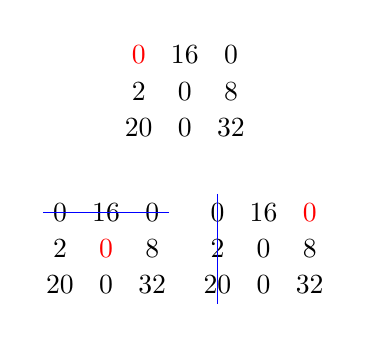
\begin{tikzpicture}
\matrix (A) [matrix of math nodes] at (0,0)
{ \node[red] {0}; & 16 & 0 \\
2 & 0 & 8 \\
20 & 0 & 32 \\
}; 
\matrix (B) [matrix of math nodes] at (-1,-2)
{ 0 & 16 & 0 \\
2 & \node[red] {0}; & 8 \\
20 & 0 & 32 \\
};
\matrix (C) [matrix of math nodes] at (1,-2)
{ 0 & 16 & \node[red]{0}; \\
2 & 0 & 8 \\
20 & 0 & 32 \\
};
\draw[blue] (B-1-1.west) -- (B-1-3.east);
\draw[blue] (C-1-1.north) -- (C-3-1.south);
\end{tikzpicture}
\end{document}
